% Options for packages loaded elsewhere
\PassOptionsToPackage{unicode}{hyperref}
\PassOptionsToPackage{hyphens}{url}
%
\documentclass[
]{article}
\usepackage{amsmath,amssymb}
\usepackage{lmodern}
\usepackage{iftex}
\ifPDFTeX
  \usepackage[T1]{fontenc}
  \usepackage[utf8]{inputenc}
  \usepackage{textcomp} % provide euro and other symbols
\else % if luatex or xetex
  \usepackage{unicode-math}
  \defaultfontfeatures{Scale=MatchLowercase}
  \defaultfontfeatures[\rmfamily]{Ligatures=TeX,Scale=1}
\fi
% Use upquote if available, for straight quotes in verbatim environments
\IfFileExists{upquote.sty}{\usepackage{upquote}}{}
\IfFileExists{microtype.sty}{% use microtype if available
  \usepackage[]{microtype}
  \UseMicrotypeSet[protrusion]{basicmath} % disable protrusion for tt fonts
}{}
\makeatletter
\@ifundefined{KOMAClassName}{% if non-KOMA class
  \IfFileExists{parskip.sty}{%
    \usepackage{parskip}
  }{% else
    \setlength{\parindent}{0pt}
    \setlength{\parskip}{6pt plus 2pt minus 1pt}}
}{% if KOMA class
  \KOMAoptions{parskip=half}}
\makeatother
\usepackage{xcolor}
\usepackage[margin=1in]{geometry}
\usepackage{color}
\usepackage{fancyvrb}
\newcommand{\VerbBar}{|}
\newcommand{\VERB}{\Verb[commandchars=\\\{\}]}
\DefineVerbatimEnvironment{Highlighting}{Verbatim}{commandchars=\\\{\}}
% Add ',fontsize=\small' for more characters per line
\usepackage{framed}
\definecolor{shadecolor}{RGB}{248,248,248}
\newenvironment{Shaded}{\begin{snugshade}}{\end{snugshade}}
\newcommand{\AlertTok}[1]{\textcolor[rgb]{0.94,0.16,0.16}{#1}}
\newcommand{\AnnotationTok}[1]{\textcolor[rgb]{0.56,0.35,0.01}{\textbf{\textit{#1}}}}
\newcommand{\AttributeTok}[1]{\textcolor[rgb]{0.77,0.63,0.00}{#1}}
\newcommand{\BaseNTok}[1]{\textcolor[rgb]{0.00,0.00,0.81}{#1}}
\newcommand{\BuiltInTok}[1]{#1}
\newcommand{\CharTok}[1]{\textcolor[rgb]{0.31,0.60,0.02}{#1}}
\newcommand{\CommentTok}[1]{\textcolor[rgb]{0.56,0.35,0.01}{\textit{#1}}}
\newcommand{\CommentVarTok}[1]{\textcolor[rgb]{0.56,0.35,0.01}{\textbf{\textit{#1}}}}
\newcommand{\ConstantTok}[1]{\textcolor[rgb]{0.00,0.00,0.00}{#1}}
\newcommand{\ControlFlowTok}[1]{\textcolor[rgb]{0.13,0.29,0.53}{\textbf{#1}}}
\newcommand{\DataTypeTok}[1]{\textcolor[rgb]{0.13,0.29,0.53}{#1}}
\newcommand{\DecValTok}[1]{\textcolor[rgb]{0.00,0.00,0.81}{#1}}
\newcommand{\DocumentationTok}[1]{\textcolor[rgb]{0.56,0.35,0.01}{\textbf{\textit{#1}}}}
\newcommand{\ErrorTok}[1]{\textcolor[rgb]{0.64,0.00,0.00}{\textbf{#1}}}
\newcommand{\ExtensionTok}[1]{#1}
\newcommand{\FloatTok}[1]{\textcolor[rgb]{0.00,0.00,0.81}{#1}}
\newcommand{\FunctionTok}[1]{\textcolor[rgb]{0.00,0.00,0.00}{#1}}
\newcommand{\ImportTok}[1]{#1}
\newcommand{\InformationTok}[1]{\textcolor[rgb]{0.56,0.35,0.01}{\textbf{\textit{#1}}}}
\newcommand{\KeywordTok}[1]{\textcolor[rgb]{0.13,0.29,0.53}{\textbf{#1}}}
\newcommand{\NormalTok}[1]{#1}
\newcommand{\OperatorTok}[1]{\textcolor[rgb]{0.81,0.36,0.00}{\textbf{#1}}}
\newcommand{\OtherTok}[1]{\textcolor[rgb]{0.56,0.35,0.01}{#1}}
\newcommand{\PreprocessorTok}[1]{\textcolor[rgb]{0.56,0.35,0.01}{\textit{#1}}}
\newcommand{\RegionMarkerTok}[1]{#1}
\newcommand{\SpecialCharTok}[1]{\textcolor[rgb]{0.00,0.00,0.00}{#1}}
\newcommand{\SpecialStringTok}[1]{\textcolor[rgb]{0.31,0.60,0.02}{#1}}
\newcommand{\StringTok}[1]{\textcolor[rgb]{0.31,0.60,0.02}{#1}}
\newcommand{\VariableTok}[1]{\textcolor[rgb]{0.00,0.00,0.00}{#1}}
\newcommand{\VerbatimStringTok}[1]{\textcolor[rgb]{0.31,0.60,0.02}{#1}}
\newcommand{\WarningTok}[1]{\textcolor[rgb]{0.56,0.35,0.01}{\textbf{\textit{#1}}}}
\usepackage{graphicx}
\makeatletter
\def\maxwidth{\ifdim\Gin@nat@width>\linewidth\linewidth\else\Gin@nat@width\fi}
\def\maxheight{\ifdim\Gin@nat@height>\textheight\textheight\else\Gin@nat@height\fi}
\makeatother
% Scale images if necessary, so that they will not overflow the page
% margins by default, and it is still possible to overwrite the defaults
% using explicit options in \includegraphics[width, height, ...]{}
\setkeys{Gin}{width=\maxwidth,height=\maxheight,keepaspectratio}
% Set default figure placement to htbp
\makeatletter
\def\fps@figure{htbp}
\makeatother
\setlength{\emergencystretch}{3em} % prevent overfull lines
\providecommand{\tightlist}{%
  \setlength{\itemsep}{0pt}\setlength{\parskip}{0pt}}
\setcounter{secnumdepth}{-\maxdimen} % remove section numbering
\ifLuaTeX
  \usepackage{selnolig}  % disable illegal ligatures
\fi
\IfFileExists{bookmark.sty}{\usepackage{bookmark}}{\usepackage{hyperref}}
\IfFileExists{xurl.sty}{\usepackage{xurl}}{} % add URL line breaks if available
\urlstyle{same} % disable monospaced font for URLs
\hypersetup{
  pdftitle={Applications of MINMI and GBRM},
  pdfauthor={Victor Tsang (z5209633)},
  hidelinks,
  pdfcreator={LaTeX via pandoc}}

\title{Applications of MINMI and GBRM}
\author{Victor Tsang (z5209633)}
\date{2022-11-08}

\begin{document}
\maketitle

\hypertarget{load-functions}{%
\subsection{Load functions}\label{load-functions}}

\begin{Shaded}
\begin{Highlighting}[]
\FunctionTok{library}\NormalTok{(tidyverse)}
\end{Highlighting}
\end{Shaded}

\begin{verbatim}
## Warning: package 'tidyverse' was built under R version 4.2.1
\end{verbatim}

\begin{verbatim}
## -- Attaching packages --------------------------------------- tidyverse 1.3.2 --
## v ggplot2 3.3.6      v purrr   0.3.4 
## v tibble  3.1.8      v dplyr   1.0.10
## v tidyr   1.2.1      v stringr 1.4.1 
## v readr   2.1.2      v forcats 0.5.2
\end{verbatim}

\begin{verbatim}
## Warning: package 'tibble' was built under R version 4.2.1
\end{verbatim}

\begin{verbatim}
## Warning: package 'tidyr' was built under R version 4.2.1
\end{verbatim}

\begin{verbatim}
## Warning: package 'readr' was built under R version 4.2.1
\end{verbatim}

\begin{verbatim}
## Warning: package 'dplyr' was built under R version 4.2.1
\end{verbatim}

\begin{verbatim}
## Warning: package 'stringr' was built under R version 4.2.1
\end{verbatim}

\begin{verbatim}
## Warning: package 'forcats' was built under R version 4.2.1
\end{verbatim}

\begin{verbatim}
## -- Conflicts ------------------------------------------ tidyverse_conflicts() --
## x dplyr::filter() masks stats::filter()
## x dplyr::lag()    masks stats::lag()
\end{verbatim}

\begin{Shaded}
\begin{Highlighting}[]
\FunctionTok{library}\NormalTok{(readxl)}
\end{Highlighting}
\end{Shaded}

\begin{verbatim}
## Warning: package 'readxl' was built under R version 4.2.1
\end{verbatim}

\begin{Shaded}
\begin{Highlighting}[]
\FunctionTok{source}\NormalTok{(}\StringTok{"../src/garthwaite{-}robbins{-}munro{-}functions.R"}\NormalTok{)}
\FunctionTok{source}\NormalTok{(}\StringTok{"../src/minmi{-}functions.R"}\NormalTok{)}
\end{Highlighting}
\end{Shaded}

\begin{verbatim}
## 
## Attaching package: 'extraDistr'
## 
## The following object is masked from 'package:purrr':
## 
##     rdunif
\end{verbatim}

\begin{Shaded}
\begin{Highlighting}[]
\CommentTok{\# source("../src/GRIWM.R")}
\FunctionTok{source}\NormalTok{(}\StringTok{"../src/simulated{-}inversion.R"}\NormalTok{)}
\end{Highlighting}
\end{Shaded}

\begin{verbatim}
## Loading required package: nlme
## 
## Attaching package: 'nlme'
## 
## The following object is masked from 'package:dplyr':
## 
##     collapse
## 
## This is mgcv 1.8-40. For overview type 'help("mgcv-package")'.
\end{verbatim}

\begin{Shaded}
\begin{Highlighting}[]
\FunctionTok{theme\_set}\NormalTok{(}\FunctionTok{theme\_bw}\NormalTok{())}

\NormalTok{alpha }\OtherTok{=} \FloatTok{0.05}
\end{Highlighting}
\end{Shaded}

\hypertarget{import-data}{%
\subsection{Import Data}\label{import-data}}

\begin{Shaded}
\begin{Highlighting}[]
\NormalTok{cave\_bear }\OtherTok{=} \FunctionTok{read\_excel}\NormalTok{(}\AttributeTok{path=}\StringTok{\textquotesingle{}../data/fossildata.xlsx\textquotesingle{}}\NormalTok{,}
                     \AttributeTok{sheet=}\StringTok{"Ursus.spe.Eur.ext"}\NormalTok{, }
                     \AttributeTok{range=}\StringTok{"M3:N33"}\NormalTok{, }
                     \AttributeTok{col\_names=}\FunctionTok{c}\NormalTok{(}\StringTok{"age"}\NormalTok{, }\StringTok{"sd"}\NormalTok{), }
                     \AttributeTok{col\_types=}\FunctionTok{c}\NormalTok{(}\StringTok{\textquotesingle{}numeric\textquotesingle{}}\NormalTok{, }\StringTok{\textquotesingle{}numeric\textquotesingle{}}\NormalTok{))}

\NormalTok{mammoth }\OtherTok{=} \FunctionTok{read\_excel}\NormalTok{(}\AttributeTok{path=}\StringTok{\textquotesingle{}../data/fossildata.xlsx\textquotesingle{}}\NormalTok{,}
                     \AttributeTok{sheet=}\StringTok{"Mammoths Eurasian"}\NormalTok{, }
                     \AttributeTok{range=}\StringTok{"M3:N205"}\NormalTok{, }
                     \AttributeTok{col\_names=}\FunctionTok{c}\NormalTok{(}\StringTok{"age"}\NormalTok{, }\StringTok{"sd"}\NormalTok{), }
                     \AttributeTok{col\_types=}\FunctionTok{c}\NormalTok{(}\StringTok{\textquotesingle{}numeric\textquotesingle{}}\NormalTok{, }\StringTok{\textquotesingle{}numeric\textquotesingle{}}\NormalTok{))}

\NormalTok{megaloceros }\OtherTok{=} \FunctionTok{read\_excel}\NormalTok{(}\AttributeTok{path=}\StringTok{\textquotesingle{}../data/fossildata.xlsx\textquotesingle{}}\NormalTok{,}
                     \AttributeTok{sheet=}\StringTok{"Megaloceros"}\NormalTok{, }
                     \AttributeTok{range=}\StringTok{"M3:N48"}\NormalTok{, }
                     \AttributeTok{col\_names=}\FunctionTok{c}\NormalTok{(}\StringTok{"age"}\NormalTok{, }\StringTok{"sd"}\NormalTok{), }
                     \AttributeTok{col\_types=}\FunctionTok{c}\NormalTok{(}\StringTok{\textquotesingle{}numeric\textquotesingle{}}\NormalTok{, }\StringTok{\textquotesingle{}numeric\textquotesingle{}}\NormalTok{))}

\NormalTok{neanderthal }\OtherTok{=} \FunctionTok{read\_excel}\NormalTok{(}\AttributeTok{path=}\StringTok{\textquotesingle{}../data/fossildata.xlsx\textquotesingle{}}\NormalTok{,}
                     \AttributeTok{sheet=}\StringTok{"NeandertalEur"}\NormalTok{, }
                     \AttributeTok{range=}\StringTok{"M3:N147"}\NormalTok{, }
                     \AttributeTok{col\_names=}\FunctionTok{c}\NormalTok{(}\StringTok{"age"}\NormalTok{, }\StringTok{"sd"}\NormalTok{), }
                     \AttributeTok{col\_types=}\FunctionTok{c}\NormalTok{(}\StringTok{\textquotesingle{}numeric\textquotesingle{}}\NormalTok{, }\StringTok{\textquotesingle{}numeric\textquotesingle{}}\NormalTok{))}

\NormalTok{bison }\OtherTok{=} \FunctionTok{read\_excel}\NormalTok{(}\AttributeTok{path=}\StringTok{\textquotesingle{}../data/fossildata.xlsx\textquotesingle{}}\NormalTok{,}
                     \AttributeTok{sheet=}\StringTok{"BisPriscus.ext"}\NormalTok{, }
                     \AttributeTok{range=}\StringTok{"M3:N15"}\NormalTok{, }
                     \AttributeTok{col\_names=}\FunctionTok{c}\NormalTok{(}\StringTok{"age"}\NormalTok{, }\StringTok{"sd"}\NormalTok{), }
                     \AttributeTok{col\_types=}\FunctionTok{c}\NormalTok{(}\StringTok{\textquotesingle{}numeric\textquotesingle{}}\NormalTok{, }\StringTok{\textquotesingle{}numeric\textquotesingle{}}\NormalTok{))}

\NormalTok{jelephant }\OtherTok{=} \FunctionTok{read\_excel}\NormalTok{(}\AttributeTok{path=}\StringTok{\textquotesingle{}../data/fossildata.xlsx\textquotesingle{}}\NormalTok{,}
                     \AttributeTok{sheet=}\StringTok{"Paleolox.Japan"}\NormalTok{, }
                     \AttributeTok{range=}\StringTok{"M3:N13"}\NormalTok{, }
                     \AttributeTok{col\_names=}\FunctionTok{c}\NormalTok{(}\StringTok{"age"}\NormalTok{, }\StringTok{"sd"}\NormalTok{), }
                     \AttributeTok{col\_types=}\FunctionTok{c}\NormalTok{(}\StringTok{\textquotesingle{}numeric\textquotesingle{}}\NormalTok{, }\StringTok{\textquotesingle{}numeric\textquotesingle{}}\NormalTok{))}

\NormalTok{cave\_hyena }\OtherTok{=} \FunctionTok{read\_excel}\NormalTok{(}\AttributeTok{path=}\StringTok{\textquotesingle{}../data/fossildata.xlsx\textquotesingle{}}\NormalTok{,}
                     \AttributeTok{sheet=}\StringTok{"CrocCroc.Eur"}\NormalTok{, }
                     \AttributeTok{range=}\StringTok{"M3:N81"}\NormalTok{, }
                     \AttributeTok{col\_names=}\FunctionTok{c}\NormalTok{(}\StringTok{"age"}\NormalTok{, }\StringTok{"sd"}\NormalTok{), }
                     \AttributeTok{col\_types=}\FunctionTok{c}\NormalTok{(}\StringTok{\textquotesingle{}numeric\textquotesingle{}}\NormalTok{, }\StringTok{\textquotesingle{}numeric\textquotesingle{}}\NormalTok{))}

\NormalTok{tmp }\OtherTok{=} \FunctionTok{rbind}\NormalTok{(}\FunctionTok{data.frame}\NormalTok{(}\AttributeTok{age=}\NormalTok{cave\_bear}\SpecialCharTok{$}\NormalTok{age, }\AttributeTok{dataset=}\StringTok{"Cave Bear"}\NormalTok{),}
            \FunctionTok{data.frame}\NormalTok{(}\AttributeTok{age=}\NormalTok{bison}\SpecialCharTok{$}\NormalTok{age, }\AttributeTok{dataset=}\StringTok{"Steppe Bison"}\NormalTok{),}
            \FunctionTok{data.frame}\NormalTok{(}\AttributeTok{age=}\NormalTok{mammoth}\SpecialCharTok{$}\NormalTok{age, }\AttributeTok{dataset=}\StringTok{"Eurasian Mammoth"}\NormalTok{),}
            \FunctionTok{data.frame}\NormalTok{(}\AttributeTok{age=}\NormalTok{cave\_hyena}\SpecialCharTok{$}\NormalTok{age, }\AttributeTok{dataset=}\StringTok{"Cave Hyena"}\NormalTok{))}
\end{Highlighting}
\end{Shaded}

\hypertarget{histograms}{%
\subsection{Histograms}\label{histograms}}

\begin{Shaded}
\begin{Highlighting}[]
\NormalTok{p }\OtherTok{=}\NormalTok{ tmp }\SpecialCharTok{\%\textgreater{}\%} \FunctionTok{ggplot}\NormalTok{(}\FunctionTok{aes}\NormalTok{(}\AttributeTok{x=}\NormalTok{age)) }\SpecialCharTok{+}
  \FunctionTok{geom\_histogram}\NormalTok{(}\AttributeTok{position=}\StringTok{"identity"}\NormalTok{, }\AttributeTok{color=}\StringTok{"black"}\NormalTok{, }\AttributeTok{fill=}\StringTok{"grey"}\NormalTok{, }\AttributeTok{bins=}\DecValTok{7}\NormalTok{) }\SpecialCharTok{+}
  \FunctionTok{facet\_wrap}\NormalTok{(dataset }\SpecialCharTok{\textasciitilde{}}\NormalTok{ ., }\AttributeTok{scale=}\StringTok{"free"}\NormalTok{, }\AttributeTok{nrow=}\DecValTok{1}\NormalTok{)}

\NormalTok{p}
\end{Highlighting}
\end{Shaded}

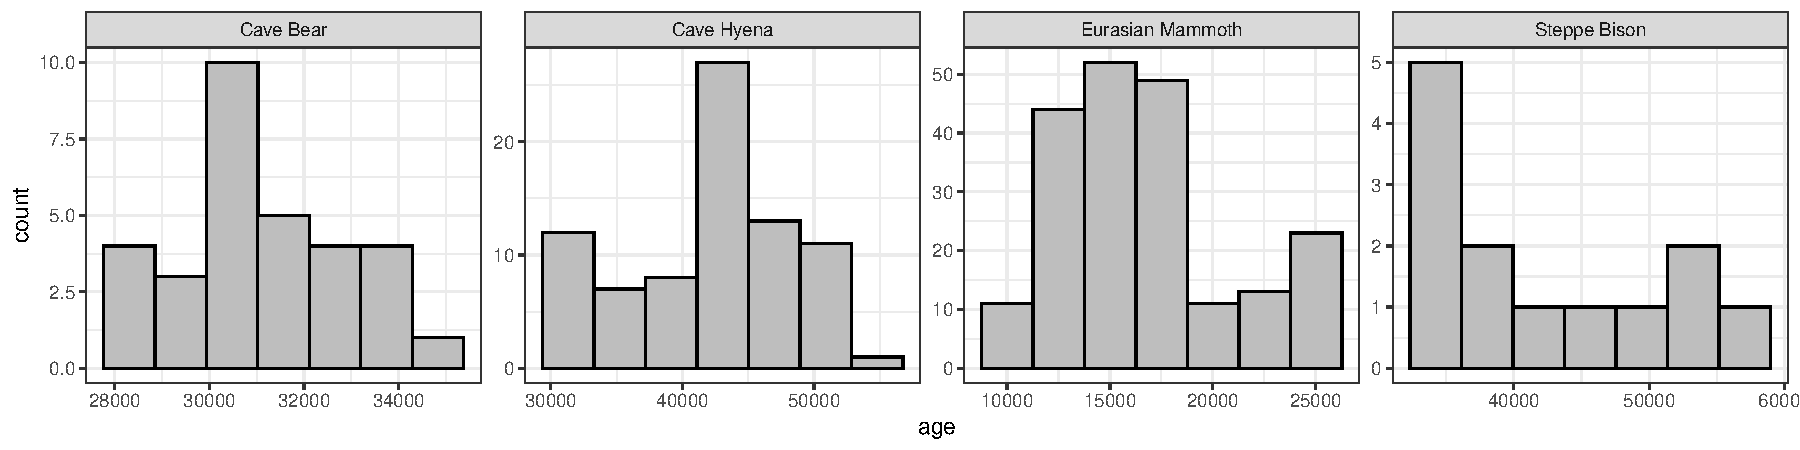
\includegraphics{applications_files/figure-latex/unnamed-chunk-3-1.pdf}

\begin{Shaded}
\begin{Highlighting}[]
\FunctionTok{ggsave}\NormalTok{(}\AttributeTok{file=}\StringTok{"../figures/applications{-}hists.svg"}\NormalTok{, }\AttributeTok{plot=}\NormalTok{p, }\AttributeTok{width=}\DecValTok{12}\NormalTok{, }\AttributeTok{height=}\DecValTok{3}\NormalTok{)}
\end{Highlighting}
\end{Shaded}

\begin{Shaded}
\begin{Highlighting}[]
\NormalTok{estimate\_extinction }\OtherTok{=} \ControlFlowTok{function}\NormalTok{ (dates, sd, K, theta.test\_vec, }\AttributeTok{alpha=}\FloatTok{0.05}\NormalTok{, label) \{}
\NormalTok{  SIUGM.results }\OtherTok{=} \FunctionTok{simulated\_inversion}\NormalTok{(}\AttributeTok{alpha=}\NormalTok{alpha, }\AttributeTok{dates=}\NormalTok{dates, }\AttributeTok{sd=}\NormalTok{sd, }\AttributeTok{K=}\NormalTok{K, }\AttributeTok{theta.test\_vec =}\NormalTok{ theta.test\_vec, }\AttributeTok{return\_model=}\NormalTok{T)}
\NormalTok{  SIUGM }\OtherTok{=} \FunctionTok{list}\NormalTok{(}\AttributeTok{lower =}\NormalTok{ SIUGM.results}\SpecialCharTok{$}\NormalTok{lower,}
               \AttributeTok{point =}\NormalTok{ SIUGM.results}\SpecialCharTok{$}\NormalTok{point,}
               \AttributeTok{upper =}\NormalTok{ SIUGM.results}\SpecialCharTok{$}\NormalTok{upper,}
               \AttributeTok{method =} \StringTok{"SI{-}UGM"}\NormalTok{)}
  
\NormalTok{  MINMI }\OtherTok{=} \FunctionTok{estimate\_extinction.minmi}\NormalTok{(}\AttributeTok{W =}\NormalTok{ dates, }\AttributeTok{sd=}\NormalTok{sd, }\AttributeTok{level=}\DecValTok{1}\SpecialCharTok{{-}}\NormalTok{alpha, }\AttributeTok{K=}\NormalTok{K)}
\NormalTok{  MINMI}\SpecialCharTok{$}\NormalTok{method }\OtherTok{=} \StringTok{"MINMI"}
  
\NormalTok{  SIRM }\OtherTok{=} \FunctionTok{estimate\_CI.rm}\NormalTok{(}\AttributeTok{W =}\NormalTok{ dates, }\AttributeTok{K=}\NormalTok{K, }\AttributeTok{alpha=}\NormalTok{alpha, }\AttributeTok{max\_iter=}\DecValTok{3000}\NormalTok{, }\AttributeTok{eps.mean=}\DecValTok{0}\NormalTok{, }\AttributeTok{eps.sigma=}\FunctionTok{mean}\NormalTok{(sd), }\AttributeTok{.model =}\NormalTok{ SIUGM.results}\SpecialCharTok{$}\NormalTok{model, }\AttributeTok{.CI\_estimates =} \FunctionTok{list}\NormalTok{(}\AttributeTok{lower=}\NormalTok{SIUGM.results}\SpecialCharTok{$}\NormalTok{lower, }\AttributeTok{upper=}\NormalTok{SIUGM.results}\SpecialCharTok{$}\NormalTok{upper))}
\NormalTok{  SIRM}\SpecialCharTok{$}\NormalTok{method }\OtherTok{=} \StringTok{"SI{-}RM"}
  
\NormalTok{  estimates }\OtherTok{=} \FunctionTok{data.frame}\NormalTok{(}
    \AttributeTok{method =} \FunctionTok{factor}\NormalTok{(),}
    \AttributeTok{lower =} \FunctionTok{numeric}\NormalTok{(),}
    \AttributeTok{upper =} \FunctionTok{numeric}\NormalTok{(),}
    \AttributeTok{point =} \FunctionTok{numeric}\NormalTok{(),}
    \AttributeTok{n =} \FunctionTok{numeric}\NormalTok{(),}
    \AttributeTok{sigma =} \FunctionTok{numeric}\NormalTok{(),}
    \AttributeTok{dataset =} \FunctionTok{factor}\NormalTok{()}
\NormalTok{  )}
\NormalTok{  estimates }\OtherTok{=} \FunctionTok{rbind}\NormalTok{(estimates, MINMI, SIUGM, SIRM)}
\NormalTok{  estimates}\SpecialCharTok{$}\NormalTok{n }\OtherTok{=} \FunctionTok{length}\NormalTok{(dates)}
\NormalTok{  estimates}\SpecialCharTok{$}\NormalTok{sigma }\OtherTok{=} \FunctionTok{mean}\NormalTok{(sd)}
\NormalTok{  estimates}\SpecialCharTok{$}\NormalTok{dataset }\OtherTok{=} \FunctionTok{paste0}\NormalTok{(label, }\StringTok{" (n="}\NormalTok{, }\FunctionTok{length}\NormalTok{(dates), }\StringTok{")"}\NormalTok{)}
  \FunctionTok{return}\NormalTok{(estimates)}
\NormalTok{\} }
\end{Highlighting}
\end{Shaded}

\hypertarget{cave-bear}{%
\subsection{Cave Bear}\label{cave-bear}}

\begin{Shaded}
\begin{Highlighting}[]
\NormalTok{cave\_bear.K }\OtherTok{=} \DecValTok{34000}
\NormalTok{cave\_bear }\OtherTok{=}\NormalTok{ cave\_bear[cave\_bear}\SpecialCharTok{$}\NormalTok{age }\SpecialCharTok{\textless{}}\NormalTok{ cave\_bear.K, ]}
\NormalTok{cave\_bear.thetas }\OtherTok{=} \FunctionTok{seq}\NormalTok{(}\DecValTok{22000}\NormalTok{, }\DecValTok{29000}\NormalTok{)}

\NormalTok{cave\_bear.estimates }\OtherTok{=} \FunctionTok{estimate\_extinction}\NormalTok{(}\AttributeTok{dates=}\NormalTok{cave\_bear}\SpecialCharTok{$}\NormalTok{age, }\AttributeTok{sd=}\NormalTok{cave\_bear}\SpecialCharTok{$}\NormalTok{sd, }\AttributeTok{K=}\NormalTok{cave\_bear.K, }\AttributeTok{theta.test\_vec =}\NormalTok{ cave\_bear.thetas, }\AttributeTok{label=}\StringTok{"Cave Bear"}\NormalTok{)}
\NormalTok{cave\_bear.estimates}
\end{Highlighting}
\end{Shaded}

\begin{verbatim}
##      point    lower    upper method  n   sigma          dataset
## 1 27946.58 26909.00 29097.54  MINMI 30 672.775 Cave Bear (n=30)
## 2 28186.53 27066.01 29331.62 SI-UGM 30 672.775 Cave Bear (n=30)
## 3 27832.00 26334.41 28648.92  SI-RM 30 672.775 Cave Bear (n=30)
\end{verbatim}

\begin{Shaded}
\begin{Highlighting}[]
\FunctionTok{ggplot}\NormalTok{(}\AttributeTok{data=}\NormalTok{cave\_bear.estimates, }\FunctionTok{aes}\NormalTok{(}\AttributeTok{colour=}\NormalTok{method)) }\SpecialCharTok{+}
  \FunctionTok{geom\_errorbar}\NormalTok{(}\FunctionTok{aes}\NormalTok{(}\AttributeTok{x=}\NormalTok{method, }\AttributeTok{ymin=}\NormalTok{lower, }\AttributeTok{ymax=}\NormalTok{upper)) }\SpecialCharTok{+} 
  \FunctionTok{geom\_point}\NormalTok{(}\FunctionTok{aes}\NormalTok{(}\AttributeTok{x=}\NormalTok{method, }\AttributeTok{y=}\NormalTok{point)) }\SpecialCharTok{+}
  \FunctionTok{geom\_hline}\NormalTok{(}\AttributeTok{yintercept=}\FunctionTok{min}\NormalTok{(cave\_bear}\SpecialCharTok{$}\NormalTok{age)) }\SpecialCharTok{+}
  \FunctionTok{guides}\NormalTok{(}\AttributeTok{colour=}\StringTok{"none"}\NormalTok{) }\SpecialCharTok{+}
  \FunctionTok{labs}\NormalTok{(}\AttributeTok{x=}\ConstantTok{NULL}\NormalTok{, }\AttributeTok{y=}\StringTok{"Years BP"}\NormalTok{, }\AttributeTok{title=}\StringTok{"Cave Bear Extinction (Ursus.spe.Eur.ext)"}\NormalTok{)}
\end{Highlighting}
\end{Shaded}

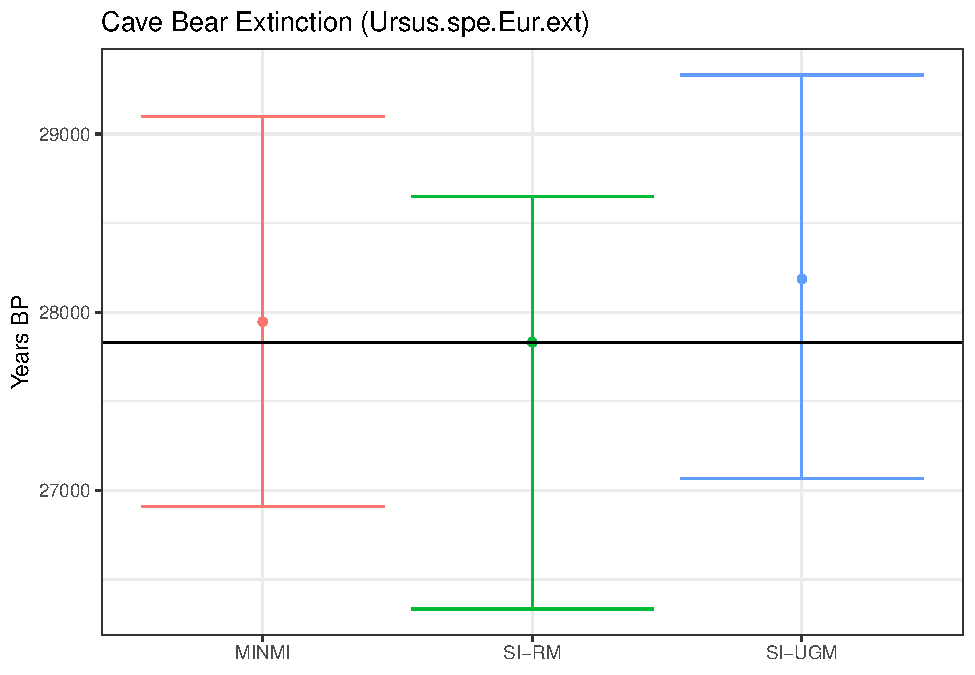
\includegraphics{applications_files/figure-latex/unnamed-chunk-5-1.pdf}

\hypertarget{eurasian-mammoth}{%
\subsection{Eurasian Mammoth}\label{eurasian-mammoth}}

\begin{Shaded}
\begin{Highlighting}[]
\NormalTok{mammoth.K }\OtherTok{=} \DecValTok{25000}
\NormalTok{mammoth }\OtherTok{=}\NormalTok{ mammoth[mammoth}\SpecialCharTok{$}\NormalTok{age }\SpecialCharTok{\textless{}}\NormalTok{ mammoth.K, ]}
\NormalTok{mammoth.thetas }\OtherTok{=} \FunctionTok{seq}\NormalTok{(}\DecValTok{4000}\NormalTok{, }\DecValTok{14000}\NormalTok{)}

\NormalTok{mammoth.estimates }\OtherTok{=} \FunctionTok{estimate\_extinction}\NormalTok{(}\AttributeTok{dates=}\NormalTok{mammoth}\SpecialCharTok{$}\NormalTok{age, }\AttributeTok{sd=}\NormalTok{mammoth}\SpecialCharTok{$}\NormalTok{sd, }\AttributeTok{K=}\NormalTok{mammoth.K, }\AttributeTok{theta.test\_vec =}\NormalTok{ mammoth.thetas, }\AttributeTok{label=}\StringTok{"Eurasian Mammoth"}\NormalTok{)}
\NormalTok{mammoth.estimates}
\end{Highlighting}
\end{Shaded}

\begin{verbatim}
##      point    lower    upper method   n    sigma                  dataset
## 1 10949.15 10578.86 11408.49  MINMI 194 281.5696 Eurasian Mammoth (n=194)
## 2 11003.50 10580.02 11426.98 SI-UGM 194 281.5696 Eurasian Mammoth (n=194)
## 3 10832.00 10246.78 11033.88  SI-RM 194 281.5696 Eurasian Mammoth (n=194)
\end{verbatim}

\begin{Shaded}
\begin{Highlighting}[]
\FunctionTok{ggplot}\NormalTok{(}\AttributeTok{data=}\NormalTok{mammoth.estimates, }\FunctionTok{aes}\NormalTok{(}\AttributeTok{colour=}\NormalTok{method)) }\SpecialCharTok{+}
  \FunctionTok{geom\_errorbar}\NormalTok{(}\FunctionTok{aes}\NormalTok{(}\AttributeTok{x=}\NormalTok{method, }\AttributeTok{ymin=}\NormalTok{lower, }\AttributeTok{ymax=}\NormalTok{upper)) }\SpecialCharTok{+} 
  \FunctionTok{geom\_point}\NormalTok{(}\FunctionTok{aes}\NormalTok{(}\AttributeTok{x=}\NormalTok{method, }\AttributeTok{y=}\NormalTok{point)) }\SpecialCharTok{+}
  \FunctionTok{guides}\NormalTok{(}\AttributeTok{colour=}\StringTok{"none"}\NormalTok{) }\SpecialCharTok{+}
  \FunctionTok{geom\_hline}\NormalTok{(}\AttributeTok{yintercept=}\FunctionTok{min}\NormalTok{(mammoth}\SpecialCharTok{$}\NormalTok{age)) }\SpecialCharTok{+}
  \FunctionTok{labs}\NormalTok{(}\AttributeTok{x=}\ConstantTok{NULL}\NormalTok{, }\AttributeTok{y=}\StringTok{"Years BP"}\NormalTok{, }\AttributeTok{title=}\StringTok{"Mammoth Extinction (MammothPrimEBer)"}\NormalTok{)}
\end{Highlighting}
\end{Shaded}

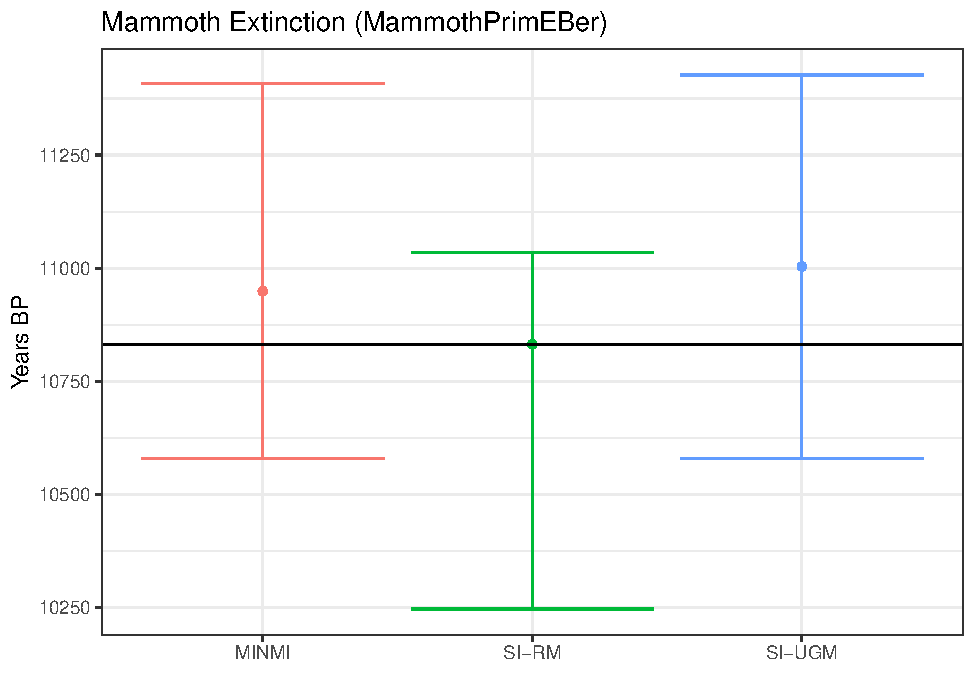
\includegraphics{applications_files/figure-latex/unnamed-chunk-6-1.pdf}

\hypertarget{giant-deer}{%
\subsection{Giant Deer}\label{giant-deer}}

\begin{Shaded}
\begin{Highlighting}[]
\NormalTok{megaloceros.K }\OtherTok{=} \DecValTok{14000}
\NormalTok{megaloceros }\OtherTok{=}\NormalTok{ megaloceros[megaloceros}\SpecialCharTok{$}\NormalTok{age }\SpecialCharTok{\textless{}}\NormalTok{ megaloceros.K, ]}
\NormalTok{megaloceros.thetas }\OtherTok{=} \FunctionTok{seq}\NormalTok{(}\DecValTok{8000}\NormalTok{, }\DecValTok{13000}\NormalTok{)}

\NormalTok{megaloceros.estimates }\OtherTok{=} \FunctionTok{estimate\_extinction}\NormalTok{(}\AttributeTok{dates=}\NormalTok{megaloceros}\SpecialCharTok{$}\NormalTok{age, }\AttributeTok{sd=}\NormalTok{megaloceros}\SpecialCharTok{$}\NormalTok{sd, }\AttributeTok{K=}\NormalTok{megaloceros.K, }\AttributeTok{theta.test\_vec =}\NormalTok{ megaloceros.thetas, }\AttributeTok{label=}\StringTok{"Giant Deer"}\NormalTok{)}
\NormalTok{megaloceros.estimates}
\end{Highlighting}
\end{Shaded}

\begin{verbatim}
##      point    lower    upper method  n  sigma           dataset
## 1 12401.21 12209.40 12586.89  MINMI 40 103.05 Giant Deer (n=40)
## 2 12466.58 12261.90 12582.28 SI-UGM 40 103.05 Giant Deer (n=40)
## 3 12402.00 12246.01 12532.00  SI-RM 40 103.05 Giant Deer (n=40)
\end{verbatim}

\begin{Shaded}
\begin{Highlighting}[]
\FunctionTok{ggplot}\NormalTok{(}\AttributeTok{data=}\NormalTok{megaloceros.estimates, }\FunctionTok{aes}\NormalTok{(}\AttributeTok{colour=}\NormalTok{method)) }\SpecialCharTok{+}
  \FunctionTok{geom\_errorbar}\NormalTok{(}\FunctionTok{aes}\NormalTok{(}\AttributeTok{x=}\NormalTok{method, }\AttributeTok{ymin=}\NormalTok{lower, }\AttributeTok{ymax=}\NormalTok{upper)) }\SpecialCharTok{+} 
  \FunctionTok{geom\_point}\NormalTok{(}\FunctionTok{aes}\NormalTok{(}\AttributeTok{x=}\NormalTok{method, }\AttributeTok{y=}\NormalTok{point)) }\SpecialCharTok{+}
  \FunctionTok{guides}\NormalTok{(}\AttributeTok{colour=}\StringTok{"none"}\NormalTok{) }\SpecialCharTok{+}
  \FunctionTok{geom\_hline}\NormalTok{(}\AttributeTok{yintercept=}\FunctionTok{min}\NormalTok{(megaloceros}\SpecialCharTok{$}\NormalTok{age)) }\SpecialCharTok{+}
  \FunctionTok{labs}\NormalTok{(}\AttributeTok{x=}\ConstantTok{NULL}\NormalTok{, }\AttributeTok{y=}\StringTok{"Years BP"}\NormalTok{, }\AttributeTok{title=}\StringTok{"Giant Deer Extinction (megaloceros)"}\NormalTok{)}
\end{Highlighting}
\end{Shaded}

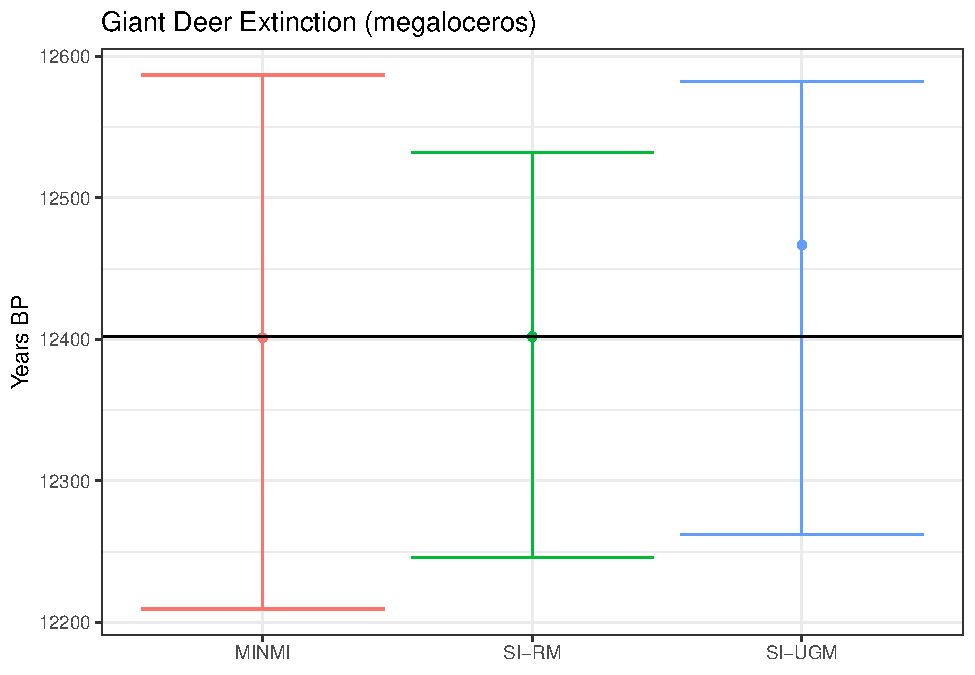
\includegraphics{applications_files/figure-latex/unnamed-chunk-7-1.pdf}

\hypertarget{neanderthal}{%
\subsection{Neanderthal}\label{neanderthal}}

\begin{Shaded}
\begin{Highlighting}[]
\NormalTok{neanderthal.K }\OtherTok{=} \DecValTok{48000}
\NormalTok{neanderthal }\OtherTok{=}\NormalTok{ neanderthal[neanderthal}\SpecialCharTok{$}\NormalTok{age }\SpecialCharTok{\textless{}}\NormalTok{ neanderthal.K, ]}
\NormalTok{neanderthal.thetas }\OtherTok{=} \FunctionTok{seq}\NormalTok{(}\DecValTok{38000}\NormalTok{, }\DecValTok{44000}\NormalTok{)}

\NormalTok{neanderthal.estimates }\OtherTok{=} \FunctionTok{estimate\_extinction}\NormalTok{(}\AttributeTok{dates=}\NormalTok{neanderthal}\SpecialCharTok{$}\NormalTok{age, }\AttributeTok{sd=}\NormalTok{neanderthal}\SpecialCharTok{$}\NormalTok{sd, }\AttributeTok{K=}\NormalTok{neanderthal.K, }\AttributeTok{theta.test\_vec =}\NormalTok{ neanderthal.thetas, }\AttributeTok{label=}\StringTok{"Neanderthal"}\NormalTok{)}
\NormalTok{neanderthal.estimates}
\end{Highlighting}
\end{Shaded}

\begin{verbatim}
##      point    lower    upper method   n    sigma             dataset
## 1 42078.54 41224.16 43228.89  MINMI 134 893.5634 Neanderthal (n=134)
## 2 42282.32 41534.67 43394.05 SI-UGM 134 893.5634 Neanderthal (n=134)
## 3 41015.00 38734.57 41414.30  SI-RM 134 893.5634 Neanderthal (n=134)
\end{verbatim}

\begin{Shaded}
\begin{Highlighting}[]
\FunctionTok{ggplot}\NormalTok{(}\AttributeTok{data=}\NormalTok{neanderthal.estimates, }\FunctionTok{aes}\NormalTok{(}\AttributeTok{colour=}\NormalTok{method)) }\SpecialCharTok{+}
  \FunctionTok{geom\_errorbar}\NormalTok{(}\FunctionTok{aes}\NormalTok{(}\AttributeTok{x=}\NormalTok{method, }\AttributeTok{ymin=}\NormalTok{lower, }\AttributeTok{ymax=}\NormalTok{upper)) }\SpecialCharTok{+} 
  \FunctionTok{geom\_point}\NormalTok{(}\FunctionTok{aes}\NormalTok{(}\AttributeTok{x=}\NormalTok{method, }\AttributeTok{y=}\NormalTok{point)) }\SpecialCharTok{+}
  \FunctionTok{guides}\NormalTok{(}\AttributeTok{colour=}\StringTok{"none"}\NormalTok{) }\SpecialCharTok{+}
  \FunctionTok{geom\_hline}\NormalTok{(}\AttributeTok{yintercept=}\FunctionTok{min}\NormalTok{(neanderthal}\SpecialCharTok{$}\NormalTok{age)) }\SpecialCharTok{+}
  \FunctionTok{labs}\NormalTok{(}\AttributeTok{x=}\ConstantTok{NULL}\NormalTok{, }\AttributeTok{y=}\StringTok{"Years BP"}\NormalTok{, }\AttributeTok{title=}\StringTok{"Neanderthal Extinction"}\NormalTok{)}
\end{Highlighting}
\end{Shaded}

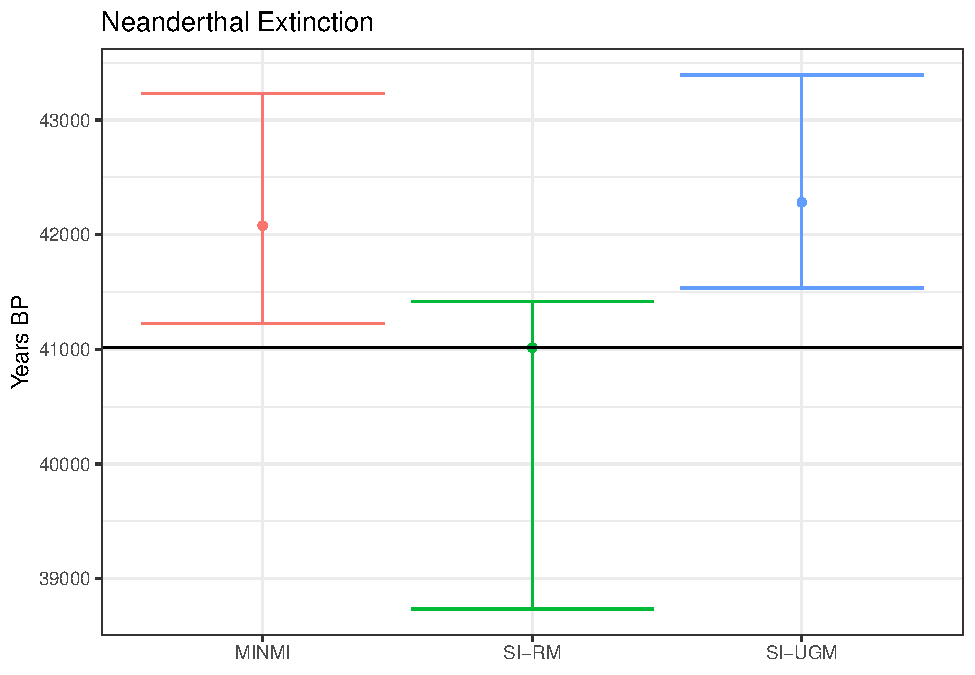
\includegraphics{applications_files/figure-latex/unnamed-chunk-8-1.pdf}

\hypertarget{steppe-bison}{%
\subsection{Steppe Bison}\label{steppe-bison}}

\begin{Shaded}
\begin{Highlighting}[]
\NormalTok{bison.K }\OtherTok{=} \DecValTok{55000}
\NormalTok{bison }\OtherTok{=}\NormalTok{ bison[bison}\SpecialCharTok{$}\NormalTok{age }\SpecialCharTok{\textless{}}\NormalTok{ bison.K, ]}
\NormalTok{bison.thetas }\OtherTok{=} \FunctionTok{seq}\NormalTok{(}\DecValTok{25000}\NormalTok{, }\DecValTok{35000}\NormalTok{)}

\NormalTok{bison.estimates }\OtherTok{=} \FunctionTok{estimate\_extinction}\NormalTok{(}\AttributeTok{dates=}\NormalTok{bison}\SpecialCharTok{$}\NormalTok{age, }\AttributeTok{sd=}\NormalTok{bison}\SpecialCharTok{$}\NormalTok{sd, }\AttributeTok{K=}\NormalTok{bison.K, }\AttributeTok{theta.test\_vec =}\NormalTok{ bison.thetas, }\AttributeTok{label=}\StringTok{"Steppe Bison"}\NormalTok{)}
\NormalTok{bison.estimates}
\end{Highlighting}
\end{Shaded}

\begin{verbatim}
##      point    lower    upper method  n    sigma             dataset
## 1 31063.08 24326.05 33808.48  MINMI 12 1123.417 Steppe Bison (n=12)
## 2 31238.77 24759.81 33911.07 SI-UGM 12 1123.417 Steppe Bison (n=12)
## 3 32489.00 30282.75 38382.76  SI-RM 12 1123.417 Steppe Bison (n=12)
\end{verbatim}

\begin{Shaded}
\begin{Highlighting}[]
\FunctionTok{ggplot}\NormalTok{(}\AttributeTok{data=}\NormalTok{bison.estimates, }\FunctionTok{aes}\NormalTok{(}\AttributeTok{colour=}\NormalTok{method)) }\SpecialCharTok{+}
  \FunctionTok{geom\_errorbar}\NormalTok{(}\FunctionTok{aes}\NormalTok{(}\AttributeTok{x=}\NormalTok{method, }\AttributeTok{ymin=}\NormalTok{lower, }\AttributeTok{ymax=}\NormalTok{upper)) }\SpecialCharTok{+} 
  \FunctionTok{geom\_point}\NormalTok{(}\FunctionTok{aes}\NormalTok{(}\AttributeTok{x=}\NormalTok{method, }\AttributeTok{y=}\NormalTok{point)) }\SpecialCharTok{+}
  \FunctionTok{guides}\NormalTok{(}\AttributeTok{colour=}\StringTok{"none"}\NormalTok{) }\SpecialCharTok{+}
  \FunctionTok{geom\_hline}\NormalTok{(}\AttributeTok{yintercept=}\FunctionTok{min}\NormalTok{(bison}\SpecialCharTok{$}\NormalTok{age)) }\SpecialCharTok{+}
  \FunctionTok{labs}\NormalTok{(}\AttributeTok{x=}\ConstantTok{NULL}\NormalTok{, }\AttributeTok{y=}\StringTok{"Years BP"}\NormalTok{, }\AttributeTok{title=}\StringTok{"Steppe Bison Extinction"}\NormalTok{)}
\end{Highlighting}
\end{Shaded}

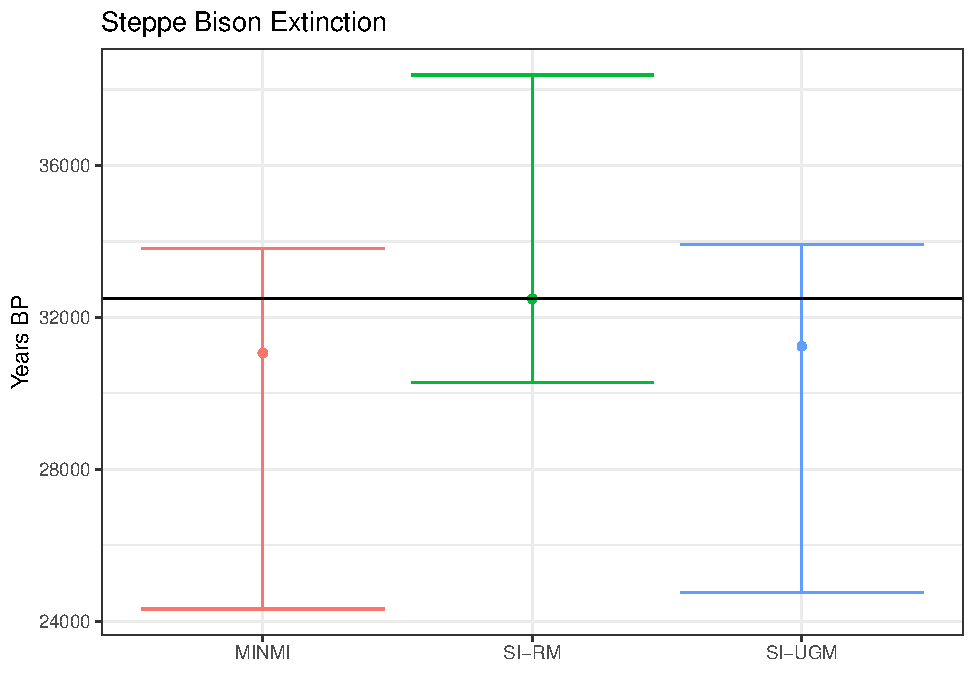
\includegraphics{applications_files/figure-latex/unnamed-chunk-9-1.pdf}

\hypertarget{japanese-elephant}{%
\subsection{Japanese Elephant}\label{japanese-elephant}}

\begin{Shaded}
\begin{Highlighting}[]
\NormalTok{jelephant.K }\OtherTok{=} \DecValTok{40000}
\NormalTok{jelephant }\OtherTok{=}\NormalTok{ jelephant[jelephant}\SpecialCharTok{$}\NormalTok{age }\SpecialCharTok{\textless{}}\NormalTok{ jelephant.K, ]}
\NormalTok{jelephant.thetas }\OtherTok{=} \FunctionTok{seq}\NormalTok{(}\DecValTok{25000}\NormalTok{, }\DecValTok{35000}\NormalTok{)}

\NormalTok{jelephant.estimates }\OtherTok{=} \FunctionTok{estimate\_extinction}\NormalTok{(}\AttributeTok{dates=}\NormalTok{jelephant}\SpecialCharTok{$}\NormalTok{age, }\AttributeTok{sd=}\NormalTok{jelephant}\SpecialCharTok{$}\NormalTok{sd, }\AttributeTok{K=}\NormalTok{jelephant.K, }\AttributeTok{theta.test\_vec =}\NormalTok{ jelephant.thetas, }\AttributeTok{label=}\StringTok{"Japanese Elephant"}\NormalTok{)}
\NormalTok{jelephant.estimates}
\end{Highlighting}
\end{Shaded}

\begin{verbatim}
##      point    lower    upper method  n   sigma                  dataset
## 1 25877.79 20880.96 27704.02  MINMI 10 708.175 Japanese Elephant (n=10)
## 2 25846.92 21631.36 27509.73 SI-UGM 10 708.175 Japanese Elephant (n=10)
## 3 26745.50 26165.03 29797.52  SI-RM 10 708.175 Japanese Elephant (n=10)
\end{verbatim}

\begin{Shaded}
\begin{Highlighting}[]
\FunctionTok{ggplot}\NormalTok{(}\AttributeTok{data=}\NormalTok{jelephant.estimates, }\FunctionTok{aes}\NormalTok{(}\AttributeTok{colour=}\NormalTok{method)) }\SpecialCharTok{+}
  \FunctionTok{geom\_errorbar}\NormalTok{(}\FunctionTok{aes}\NormalTok{(}\AttributeTok{x=}\NormalTok{method, }\AttributeTok{ymin=}\NormalTok{lower, }\AttributeTok{ymax=}\NormalTok{upper)) }\SpecialCharTok{+} 
  \FunctionTok{geom\_point}\NormalTok{(}\FunctionTok{aes}\NormalTok{(}\AttributeTok{x=}\NormalTok{method, }\AttributeTok{y=}\NormalTok{point)) }\SpecialCharTok{+}
  \FunctionTok{guides}\NormalTok{(}\AttributeTok{colour=}\StringTok{"none"}\NormalTok{) }\SpecialCharTok{+}
  \FunctionTok{geom\_hline}\NormalTok{(}\AttributeTok{yintercept=}\FunctionTok{min}\NormalTok{(jelephant}\SpecialCharTok{$}\NormalTok{age), }\AttributeTok{linetype=}\StringTok{"dashed"}\NormalTok{) }\SpecialCharTok{+}
  \FunctionTok{annotate}\NormalTok{(}\AttributeTok{geom=}\StringTok{"text"}\NormalTok{, }\AttributeTok{label=}\FunctionTok{paste}\NormalTok{(}\StringTok{"Obs. Min."}\NormalTok{, }\FunctionTok{min}\NormalTok{(jelephant}\SpecialCharTok{$}\NormalTok{age)), }\AttributeTok{x=}\DecValTok{0}\NormalTok{, }\AttributeTok{y=}\FunctionTok{min}\NormalTok{(jelephant}\SpecialCharTok{$}\NormalTok{age)}\SpecialCharTok{+}\DecValTok{250}\NormalTok{, }\AttributeTok{hjust=}\DecValTok{0}\NormalTok{, }\AttributeTok{fontface =} \StringTok{\textquotesingle{}italic\textquotesingle{}}\NormalTok{) }\SpecialCharTok{+}
  \FunctionTok{labs}\NormalTok{(}\AttributeTok{x=}\ConstantTok{NULL}\NormalTok{, }\AttributeTok{y=}\StringTok{"Years BP"}\NormalTok{, }\AttributeTok{title=}\StringTok{"Japanese Elephant Extinction"}\NormalTok{)}
\end{Highlighting}
\end{Shaded}

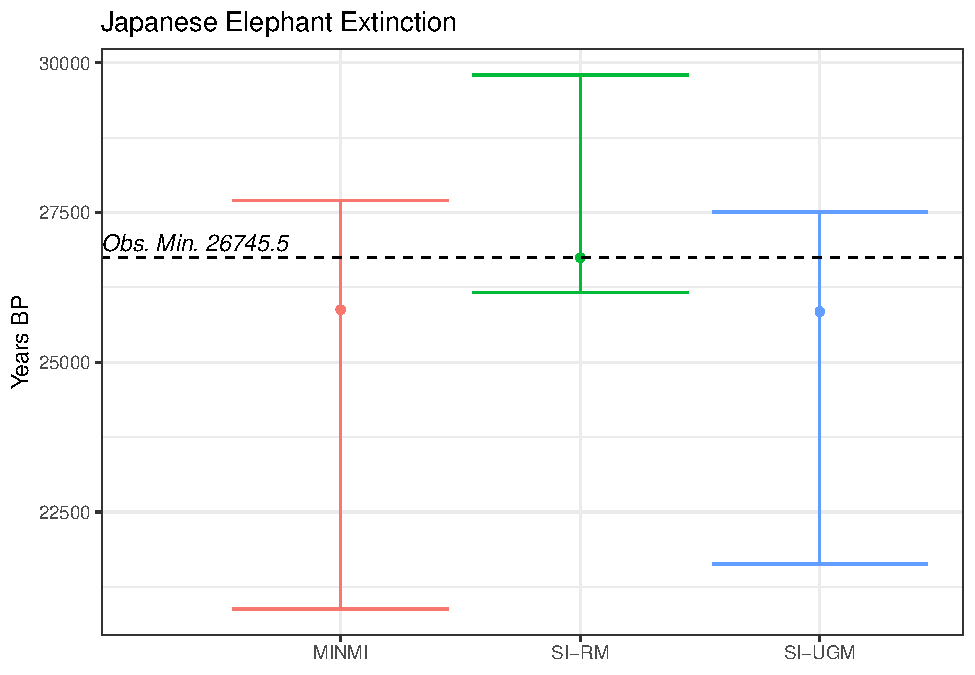
\includegraphics{applications_files/figure-latex/unnamed-chunk-10-1.pdf}

\hypertarget{cave-hyena}{%
\subsection{Cave Hyena}\label{cave-hyena}}

\begin{Shaded}
\begin{Highlighting}[]
\NormalTok{cave\_hyena.K }\OtherTok{=} \DecValTok{55000}
\NormalTok{cave\_hyena }\OtherTok{=}\NormalTok{ cave\_hyena[cave\_hyena}\SpecialCharTok{$}\NormalTok{age }\SpecialCharTok{\textless{}}\NormalTok{ cave\_hyena.K, ]}
\NormalTok{cave\_hyena.thetas }\OtherTok{=} \FunctionTok{seq}\NormalTok{(}\DecValTok{20000}\NormalTok{, }\DecValTok{30000}\NormalTok{)}

\NormalTok{cave\_hyena.estimates }\OtherTok{=} \FunctionTok{estimate\_extinction}\NormalTok{(}\AttributeTok{dates=}\NormalTok{cave\_hyena}\SpecialCharTok{$}\NormalTok{age, }\AttributeTok{sd=}\NormalTok{cave\_hyena}\SpecialCharTok{$}\NormalTok{sd, }\AttributeTok{K=}\NormalTok{cave\_hyena.K, }\AttributeTok{theta.test\_vec =}\NormalTok{ cave\_hyena.thetas, }\AttributeTok{label=}\StringTok{"Cave Hyena"}\NormalTok{)}
\NormalTok{cave\_hyena.estimates}
\end{Highlighting}
\end{Shaded}

\begin{verbatim}
##      point    lower    upper method  n    sigma           dataset
## 1 30098.38 28440.61 31812.23  MINMI 79 1117.924 Cave Hyena (n=79)
## 2 29995.93 28290.49 31701.79 SI-UGM 79 1117.924 Cave Hyena (n=79)
## 3 29465.50 28135.81 32051.25  SI-RM 79 1117.924 Cave Hyena (n=79)
\end{verbatim}

\begin{Shaded}
\begin{Highlighting}[]
\FunctionTok{ggplot}\NormalTok{(}\AttributeTok{data=}\NormalTok{cave\_hyena.estimates, }\FunctionTok{aes}\NormalTok{(}\AttributeTok{colour=}\NormalTok{method)) }\SpecialCharTok{+}
  \FunctionTok{geom\_errorbar}\NormalTok{(}\FunctionTok{aes}\NormalTok{(}\AttributeTok{x=}\NormalTok{method, }\AttributeTok{ymin=}\NormalTok{lower, }\AttributeTok{ymax=}\NormalTok{upper)) }\SpecialCharTok{+} 
  \FunctionTok{geom\_point}\NormalTok{(}\FunctionTok{aes}\NormalTok{(}\AttributeTok{x=}\NormalTok{method, }\AttributeTok{y=}\NormalTok{point)) }\SpecialCharTok{+}
  \FunctionTok{guides}\NormalTok{(}\AttributeTok{colour=}\StringTok{"none"}\NormalTok{) }\SpecialCharTok{+}
  \FunctionTok{geom\_hline}\NormalTok{(}\AttributeTok{yintercept=}\FunctionTok{min}\NormalTok{(cave\_hyena}\SpecialCharTok{$}\NormalTok{age), }\AttributeTok{linetype=}\StringTok{"dashed"}\NormalTok{) }\SpecialCharTok{+}
  \FunctionTok{annotate}\NormalTok{(}\AttributeTok{geom=}\StringTok{"text"}\NormalTok{, }\AttributeTok{label=}\FunctionTok{paste}\NormalTok{(}\StringTok{"Obs. Min."}\NormalTok{, }\FunctionTok{min}\NormalTok{(cave\_hyena}\SpecialCharTok{$}\NormalTok{age)), }\AttributeTok{x=}\DecValTok{0}\NormalTok{, }\AttributeTok{y=}\FunctionTok{min}\NormalTok{(cave\_hyena}\SpecialCharTok{$}\NormalTok{age)}\SpecialCharTok{+}\DecValTok{150}\NormalTok{, }\AttributeTok{hjust=}\DecValTok{0}\NormalTok{, }\AttributeTok{fontface =} \StringTok{\textquotesingle{}italic\textquotesingle{}}\NormalTok{) }\SpecialCharTok{+}
  \FunctionTok{labs}\NormalTok{(}\AttributeTok{x=}\ConstantTok{NULL}\NormalTok{, }\AttributeTok{y=}\StringTok{"Years BP"}\NormalTok{, }\AttributeTok{title=}\StringTok{"Cave Hyena Extinction"}\NormalTok{)}
\end{Highlighting}
\end{Shaded}

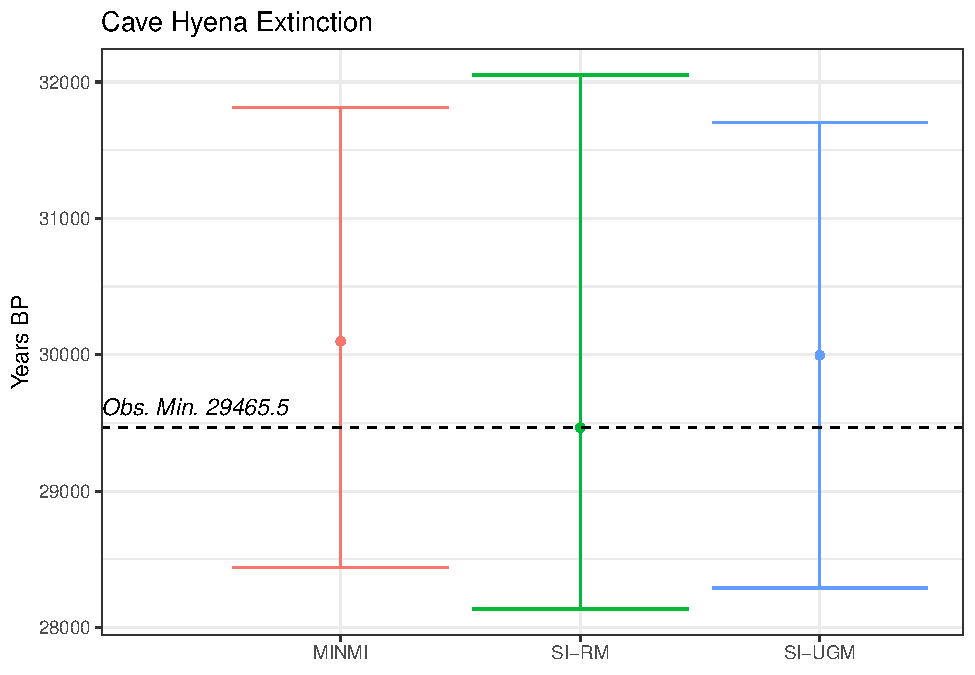
\includegraphics{applications_files/figure-latex/unnamed-chunk-11-1.pdf}

\hypertarget{combined}{%
\subsection{Combined}\label{combined}}

\begin{Shaded}
\begin{Highlighting}[]
\NormalTok{all\_results }\OtherTok{=} \FunctionTok{rbind}\NormalTok{(cave\_bear.estimates, mammoth.estimates, bison.estimates, cave\_hyena.estimates)}\CommentTok{\#, mammoth.estimates, megaloceros.estimates)}

\NormalTok{p }\OtherTok{=}\NormalTok{ all\_results }\SpecialCharTok{\%\textgreater{}\%}
  \FunctionTok{ggplot}\NormalTok{(}\FunctionTok{aes}\NormalTok{(}\AttributeTok{colour=}\NormalTok{method)) }\SpecialCharTok{+}
  \FunctionTok{geom\_errorbar}\NormalTok{(}\FunctionTok{aes}\NormalTok{(}\AttributeTok{x=}\NormalTok{method, }\AttributeTok{ymin=}\NormalTok{lower, }\AttributeTok{ymax=}\NormalTok{upper)) }\SpecialCharTok{+} 
  \FunctionTok{geom\_point}\NormalTok{(}\FunctionTok{aes}\NormalTok{(}\AttributeTok{x=}\NormalTok{method, }\AttributeTok{y=}\NormalTok{point)) }\SpecialCharTok{+}
  \FunctionTok{guides}\NormalTok{(}\AttributeTok{colour=}\StringTok{"none"}\NormalTok{) }\SpecialCharTok{+}
  \FunctionTok{labs}\NormalTok{(}\AttributeTok{x=}\ConstantTok{NULL}\NormalTok{, }\AttributeTok{y=}\StringTok{"Years (BP)"}\NormalTok{) }\SpecialCharTok{+}
  \FunctionTok{facet\_wrap}\NormalTok{(}\FunctionTok{fct\_reorder}\NormalTok{(dataset, n) }\SpecialCharTok{\textasciitilde{}}\NormalTok{ ., }\AttributeTok{nrow=}\DecValTok{1}\NormalTok{, }\AttributeTok{dir=}\StringTok{\textquotesingle{}v\textquotesingle{}}\NormalTok{)}

\NormalTok{p}
\end{Highlighting}
\end{Shaded}

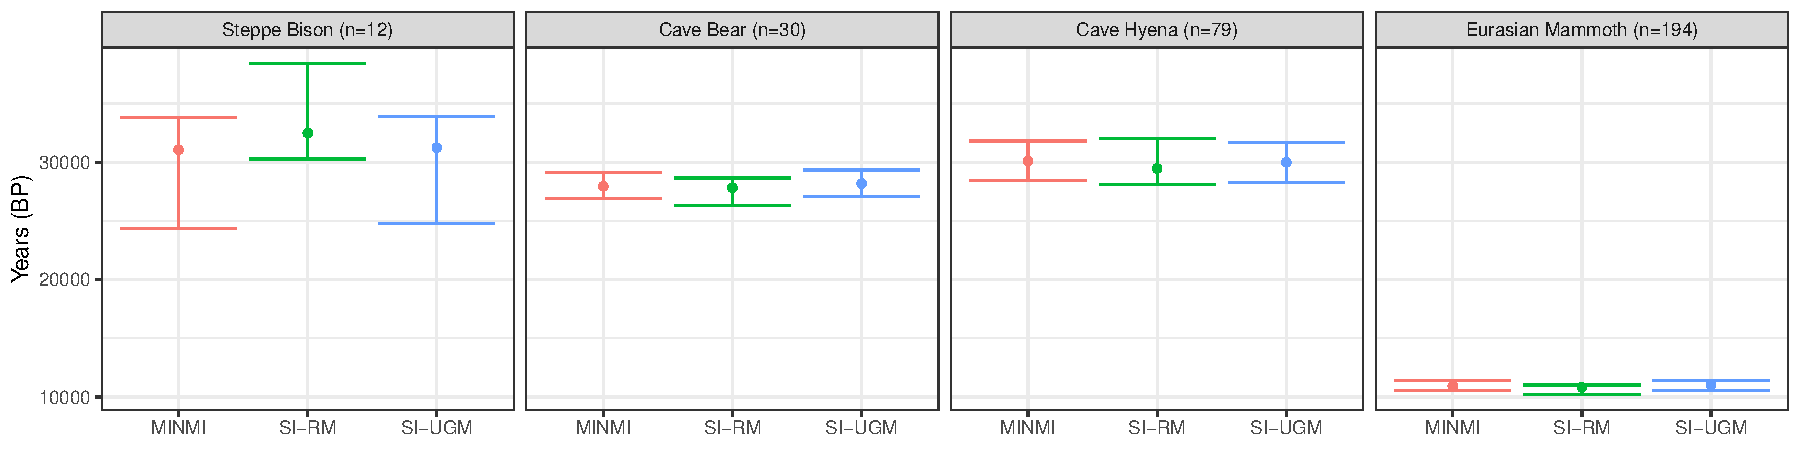
\includegraphics{applications_files/figure-latex/unnamed-chunk-12-1.pdf}

\begin{Shaded}
\begin{Highlighting}[]
\FunctionTok{ggsave}\NormalTok{(}\AttributeTok{file=}\StringTok{"../figures/applications.svg"}\NormalTok{, }\AttributeTok{plot=}\NormalTok{p, }\AttributeTok{width=}\DecValTok{12}\NormalTok{, }\AttributeTok{height=}\DecValTok{3}\NormalTok{)}
\end{Highlighting}
\end{Shaded}

\begin{Shaded}
\begin{Highlighting}[]
\FunctionTok{library}\NormalTok{(knitr)}
\end{Highlighting}
\end{Shaded}

\begin{verbatim}
## Warning: package 'knitr' was built under R version 4.2.1
\end{verbatim}

\begin{Shaded}
\begin{Highlighting}[]
\NormalTok{all\_results }\SpecialCharTok{\%\textgreater{}\%}
  \FunctionTok{mutate}\NormalTok{(}\AttributeTok{Extinction =} \FunctionTok{paste0}\NormalTok{(scales}\SpecialCharTok{::}\FunctionTok{label\_comma}\NormalTok{()(}\FunctionTok{round}\NormalTok{(point, }\DecValTok{1}\NormalTok{)), }\StringTok{" ("}\NormalTok{, scales}\SpecialCharTok{::}\FunctionTok{label\_comma}\NormalTok{()(}\FunctionTok{round}\NormalTok{(lower, }\DecValTok{1}\NormalTok{)), }\StringTok{" {-} "}\NormalTok{, scales}\SpecialCharTok{::}\FunctionTok{label\_comma}\NormalTok{()(}\FunctionTok{round}\NormalTok{(upper, }\DecValTok{1}\NormalTok{)), }\StringTok{")"}\NormalTok{),}
         \AttributeTok{Method =}\NormalTok{ method) }\SpecialCharTok{\%\textgreater{}\%}
  \FunctionTok{select}\NormalTok{(Method, dataset, Extinction) }\SpecialCharTok{\%\textgreater{}\%}
  \FunctionTok{pivot\_wider}\NormalTok{(}\AttributeTok{names\_from=}\NormalTok{dataset, }\AttributeTok{values\_from=}\NormalTok{Extinction) }\SpecialCharTok{\%\textgreater{}\%}
  \FunctionTok{kable}\NormalTok{(}\AttributeTok{booktabs=}\NormalTok{T, }\AttributeTok{format=}\StringTok{"latex"}\NormalTok{) }\SpecialCharTok{\%\textgreater{}\%}
  \FunctionTok{writeLines}\NormalTok{(}\StringTok{"../figures/table{-}applications{-}CIs.tex"}\NormalTok{)}
\end{Highlighting}
\end{Shaded}


\end{document}
